\documentclass{standalone}
\usepackage{tikz}
\usetikzlibrary{arrows.meta}


\tikzstyle{input-node}=[fill=white,circle,thick,draw]
\tikzstyle{hidden-node}=[fill=white,circle,thick,draw]
\tikzstyle{output-node}=[fill=white,circle,thick,draw]

\tikzstyle{black-line}=[draw=black,very thick]
\tikzstyle{red-line}=[draw=red,very thick]

\begin{document}
	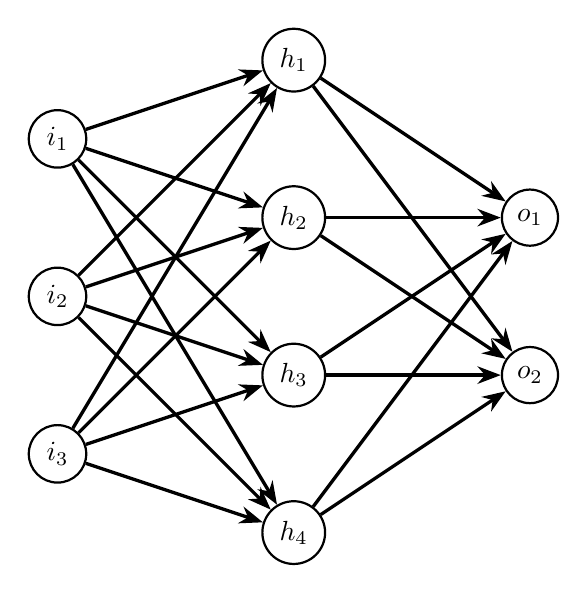
\begin{tikzpicture}
	\begin{scope}
	\node (i1)[input-node] at (0,2) {$i_1$};
	\node (i2)[input-node] at (0,0) {$i_2$};
	\node (i3)[input-node] at (0,-2) {$i_3$};
	
	\node (h1)[hidden-node] at (3,3) {$h_1$};
	\node (h2)[hidden-node] at (3,1) {$h_2$};
	\node (h3)[hidden-node] at (3,-1) {$h_3$};
	\node (h4)[hidden-node] at (3,-3) {$h_4$};
	
	\node (o1)[output-node] at (6,1) {$o_1$};
	\node (o2)[output-node] at (6,-1) {$o_2$} ;
	\end{scope}
	
	\begin{scope}[>={Stealth[black]}, every edge/.style=black-line]
	\path [->] (i1) edge node {} (h1);
	\path [->] (i1) edge node {} (h2);
	\path [->] (i1) edge node {} (h3);
	\path [->] (i1) edge node {} (h4);
	\path [->] (i2) edge node {} (h1);
	\path [->] (i2) edge node {} (h2);
	\path [->] (i2) edge node {} (h3);
	\path [->] (i2) edge node {} (h4);
	\path [->] (i3) edge node {} (h1);
	\path [->] (i3) edge node {} (h2);
	\path [->] (i3) edge node {} (h3);
	\path [->] (i3) edge node {} (h4);
	\path [->] (h1) edge node {} (o1);
	\path [->] (h1) edge node {} (o2);
	\path [->] (h2) edge node {} (o1);
	\path [->] (h2) edge node {} (o2);
	\path [->] (h3) edge node {} (o1);
	\path [->] (h3) edge node {} (o2);
	\path [->] (h4) edge node {} (o1);
	\path [->] (h4) edge node {} (o2);
	\end{scope}
	\end{tikzpicture}
\end{document}